\chapter{发送和接收数据}

通常情况下,在程序中使用套接字是因为需要向其他程序提供信息,或使用其他程序提供的信息。这并不是什么魔法:任何要交换信息的程序之间在信息的编码方式上必须达成共识(如将信息表示为位序列),以及哪个程序发送信息,什么时候和怎样接收信息都将影响程序的行为。程序间达成的这种包含了信息交换的形式和意义的共识称为协议,用来实现特定应用程序的协议叫做应用程序协议。前面章节中的回馈程序示例中的应用程序协议都过于简单:客户端和服务器的行为都不受它们之间所交换的信息内容的影响。而在绝大部分实际应用中,客户端和服务器的行为都要依赖于它们所交换的信息,因此应用程序协议通常更加复杂。 

TCP/IP协议以字节的方式传输用户数据,并没有对其进行检查和修改。这个特点使应用程序可以非常灵活地对其传输的信息进行编码。大部分的应用程序协议是根据由字段序列组成的离散信息定义的,其中每个字段中都包含了一段以位序列编码的特定的信息。应用程序协议中明确定义了信息的发送者应该怎样排列和解释这些位序列,同时还要定义接收者应该怎样解析,这样才使信息的接收者能够抽取出每个字段的意义。TCP/IP协议的唯一约束是,信息必须在块(chunks)中发送和接收,而块的长度必须是8位的倍数,因此,我们可以认为在TCP/IP协议中传输的信息是字节序列。鉴于此,我们可以进一步把传输的信息看作数字序列或数组,每个数字的取值范围是0到255。这与8位编码的二进制数值范围是一致的:00000000代表0,00000001代表1,00000010代表2,等等,最多到11111111,即255。 

如果你建立了一个程序使用套接字与其他程序交换信息,通常符合下面两种情况之一:

要么是你设计和编写了套接字的客户端和服务器端,这种情况下你能够随心所欲地定义自己的应用程序协议;

要么是你实现了一个已经存在的协议,或许是一个协议标准。

任何一种情况,在"线路上"将不同类型的信息进行字节编码和解码的基本原理还是一样的。顺便说一下,如果"线路"是由一个程序写,由另一程序读的文件,本章的所有内容对其也是适用的。 

\section{信息编码} 

	首先,我们来考虑一下简单数据类型,如int,long,char,String等,是如何通过套接字发送和接收的。从前面章节我们已经知道,传输信息时可以通过套接字将字节信息写入一个OutputStream实例中(该实例已经与一个Socket相关联),或将其封装进一个DatagramPacket实例中(该实例将由DatagramSocket发送)。然而,这些操作所能处理的唯一数据类型是字节和字节数组。作为一种强类型语言,Java需要把其他数据类型(int,String等)显式转换成字节数组。所幸的是Java的内置工具能够帮助我们完成这些转换。在第2.2.1节的TCPEchoClient.java示例程序中,我们看到过String类的getBytes()方法,该方法就是将一个Sring实例中的字符转换成字节的标准方式。在考虑数据类型转换的细节之前,我们先来看看大部分基本数据类型的表示方法。 

	\subsection{基本整型} 

		如我们所见,TCP和UDP套接字使我们能发送和接收字节序列(数组),即范围在0-255之间的整数。使用这个功能,我们可以对值更大的基本整型数据进行编码,不过发送者和接收者必须先在一些方面达成共识。一是要传输的每个整数的字节大小(size)。例如,Java程序中,int数据类型由32位表示,因此,我们可以使用4个字节来传输任意的int型变量或常量;short数据类型由16位表示,传输short类型的数据只需要两个字节;同理,传输64位的long类型数据则需要8个字节。 

		下面我们考虑如何对一个包含了4个整数的序列进行编码:一个byte型,一个short型,一个int型,以及一个long型,按照这个顺序从发送者传输到接收者。我们总共需要15个字节:第一个字节存放byte型数据,接下来两个字节存放short型数据,再后面4个字节存放int型数据,最后8个字节存放long型数据,如下所示: 

		\lstinputlisting[language=Java,firstline=1,lastline=2]{src/ch03/BruteForceCoding.txt}

		我们已经做好深入研究的准备了吗?未必。对于需要超过一个字节来表示的数据类型,我们必须知道这些字节的发送顺序。显然有两种选择:从整数的右边开始,由低位到高位地发送,即little-endian顺序;或从左边开始,由高位到低位发送,即big-endian顺序。(注意,幸运的是字节中位的顺序在实现时是以标准的方式处理的)考虑长整型数123456787654321L,其64位(以十六进制形式)表示为0x0000704885F926B1。
		
		如果我们以big-endian顺序来传输这个整数,其字节的十进制数值序列就如下所示: 

		\lstinputlisting[language=Java,firstline=12,lastline=15]{src/ch03/BruteForceCoding.txt}

		如果我们以little-endian顺序传输,则字节的十进制数组序列为: 

		\lstinputlisting[language=Java,firstline=17,lastline=20]{src/ch03/BruteForceCoding.txt}

		关键的一点是,对于任何多字节的整数,发送者和接收者必须在使用big-endian顺序还是使用little-endian顺序上达成共识。如果发送者使用了little-endian顺序来发送上述整数,而接收者以big-endian顺序对其进行接收,那么接收者将取到错误的值,它会将这个8字节序列的整数解析成12765164544669515776L。 

		Java中的ByteOrder类中有两个常量: \verb|BIG_ENDIAN| 和 \verb|LITTLE_ENDIAN| 来表示大端与小端。

		发送者和接收者需要达成共识的最后一个细节是:所传输的数值是有符号的(signed)还是无符号的(unsigned)。Java中的四种基本整型都是有符号的,它们的值以二进制补码(two's-complement)的方式存储,这是有符号数值的常用表示方式。在处理有k位的有符号数时,用二进制补码的形式表示负整数-n(1 ≤ n ≤ $2^{k-1}$),则补码的二进制值就为$2^k-n$。而对于非负整数p(0 ≤ p ≤ $2^{k-1}-1$),只是简单地用k位二进制数来表示p的值。因此,对于给定的k位,我们可以通过二进制补码来表示$-2^{k-1}$到$2^{k-1}-1$范围的值。注意,最高位(msb)标识了该数是正数(msb = 0)还是负数(msb = 1)。另外,如果使用无符号(unsigned)编码,k位可以直接表示0到$2^k-1$之间的数值。例如,32位数值0xffffffff(所有位全为1),将其解析为有符号数时,二进制补码整数表示-1;将其解析为无符号数时,它表示4294967295。由于Java并不支持无符号整型,如果要在Java中编码和解码无符号数,则需要做一点额外的工作。在此假设我们处理的都是有符号整数数据。 

		那么我们怎样才能将消息的正确值存入字节数组呢?为了清楚地展示需要做的步骤,我们将对如何使用"位操作(bit-diddling)"(移位和屏蔽)来显式编码进行介绍。示例程序BruteForceCoding.java中有一个特殊的方法encodeIntBigEndian()能够对任何值的基本类型数据进行编码。它的参数包括用来存放数值的字节数组,要进行编码的数值(表示为long型,它是最长的整型,能够保存其他整型的值),数值在字节数组中开始位置的偏移量,以及该数值写到数组中的字节数。如果我们在发送端进行了编码,那么必须能够在接收端进行解码。BruteForceCoding类同时还提供了decodeIntBigEndian()方法,用来将字节数组的子集解码到一个Java的long型整数中。 

		\lstinputlisting[language=Java,firstline=1]{src/ch03/BruteForceCoding.java}

		1. 数据项编码:第5-8行 

		2. Java中的基本整数所占字节数:第10-13行 

		3. byteArrayToDecimalString():第17-23行 

		该方法把给定数组中的每个字节作为一个无符号十进制数打印出来。BYTEMASK的作用是防止在字节数值转换成int类型时,发生符号扩展(sign-extended),即转换成无符号整型。 

		4.encodeIntBigEndian():第26-32行 

		赋值语句的右边,首先将数值向右移动,以使我们需要的字节处于该数值的低8位中。然后,将移位后的数转换成byte型,并存入字节数组的适当位置。在转换过程中,除了低8位以外,其他位都将丢弃。这个过程将根据给定数值所占字节数迭代进行。该方法还将返回存入数值后字节数组中新的偏移位置,因此我们不必做额外的工作来跟踪偏移量。 

		5. decodeIntBigEndian():第35-42行 

		根据给定数组的字节大小进行迭代,通过每次迭代的左移操作,将所取得字节的值累积到一个long型整数中。 

		6. 示例方法:第44-67行 

		准备接收整数序列的数组:第45行 

		对每项进行编码:第47-50行 

		对byte,short,int以及long型整数进行编码,并按照前面描述的顺序存入字节数组。 

		打印编码后数组的内容:第51行 

		对编码字节数组中的某些字段进行解码:第55-57行 

		解码后输出的值应该与编码前的原始值相等。 

		转换问题:第61-66行 

		在字节数组偏移量为4的位置,该字节的十进制值是245,然而,当将其作为一个有符号字节读取时,其值则为-11(回忆有符号整数的二进制补码表示方法)。如果我们将返回值直接存入一个long型整数,它只是简单地变成这个long型整数的最后一个字节,值为245。如果将返回值放入一个字节型整数,其值则为-11。到底哪个值正确取决于你的应用程序。如果你从N个字节解码后希望得到一个有符号的数值,就必须将解码结果(长的结果)存入一个刚好占用N个字节的基本整型中。如果你希望得到一个无符号的数组,就必须将解码结果存入更长的基本整型中,该整型至少要占用N+1个字节。 

		注意,在encodeIntBigEndian() 和 decodeIntBigEndian()方法的开始部分,我们可能需要做一些前提条件检测,如0 ≤ size ≤ 8 和 dst ≠ null等。你能举出需要做的其他前期检测吗? 

		运行以上程序,其输出显示了一下字节的值(以十进制形式): 

		\lstinputlisting[language=Java,firstline=31,lastline=34]{src/ch03/BruteForceCoding.txt}

		如你所见,上面的强制(brute-force)编码方法需要程序员做很多工作:要计算和命名每个数值的偏移量和大小,并要为编码过程提供合适的参数。如果没有将encodeIntBigEndian()方法提出来作为一个独立的方法,情况会更糟。基于以上原因,强制编码方法是不推荐使用的,而且Java也提供了一些更加易用的内置机制。不过,值得注意的是强制编码方法也有它的优势,除了能够对标准的Java整型进行编码外,encodeIntegerBigEndian() 方法对1到8字节的任何整数都适用--例如,如果愿意的话,你可以对一个7字节的整数进行编码。 

		构建本例中的消息的一个相对简单的方法是使用DataOutputStream类和ByteArrayOutputStream类。DataOutputStream 类允许你将基本数据类型,如上述整型,写入一个流中:它提供了writeByte(),writeShort(),writeInt(),以及writeLong()方法,这些方 按照big-endian顺序,将整数以适当大小的二进制补码的形式写到流中。ByteArrayOutputStream类获取写到流中的字节序列,并将其转换成一个字节数组。用这两个类来构建我们的消息的代码如下: 

		\lstinputlisting[language=Java,firstline=41,lastline=48]{src/ch03/BruteForceCoding.txt}

		也许你想运行这段代码,来证实它与BruteForceEncoding.java的输出结果一样。 

		讲了这么多发送方相关的内容,那么接收方将如何恢复传输的数据呢?正如你想的那样,Java中也提供了与输出工具类相似的输入工具类,分别是DataInputStream类和ByteArrayInputStream类。在后面讨论如何解析传入的消息时,我们将对这两个类的使用举例。并且,在第5章中,我们还会看到另一种方法,使用ByteBuffer类将基本数据类型转换成字节序列。 

		最后,本节的所有内容基本上也适用于BigInteger类,该类支持任意大的整数。对于基本整型,发送者和接收者必须在使用多大空间(字节数)来表示一个数值上达成共识。但是这又与使用BigInteger相矛盾,因为BigInteger可以是任意大小。一种解决方法是使用基于长度的帧,我们将在第3.3节看到这种方法。 


	\subsection{字符串和文本} 

		历史悠久的文本(可打印,即可显示的字符串)可能是用来表示信息最常用的方式。文本使用起来非常方便,因为人们习惯于处理各种各样以字符串形式表示的信息,如书本中,报纸中,以及电脑显示器上的信息。因此,只要我们指定如何对要传输的文本进行编码,我们就几乎能发送其他任何类型的数据:先将其表示成文本形式,再对文本进行编码。显然,我们可以将数字和boolean类型的数据表示成String类型,如"123478962","6.02e23","true","false"等。我们也已经看到,通过调用getBytes()方法,可以将一个字符串转换成字节数组(见TCPEchoClient.java)。当然,还有其他方法实现这个功能。 

		为了更好地理解这个过程,我们首先得将文本视为由符号和字符(characters)组成。实际上每个String实例都对应了一个字符序列(数组,char[]类型)。一个字符在Java内部表示为一个整数。例如,字符"a",即字母"a"的符号,与整数97对应;字符"X"对应了88,而符号"!"(感叹号)则对应了33。 

		在一组符号与一组整数之间的映射称为编码字符集(coded character set.)。或许你听说过ASCII编码字符集(ASCII,American Standard Code for Information Interchange,美国标准信息交换码)。ASCII码将英语字母、数字、标点符号以及一些特殊符号(不可打印字符)映射成0到127的整数。自20世纪60年代以来,ASCII码就被用来进行数据传输,甚至在今天,它也广泛应用在应用程序协议中,如HTTP(万维网所用的协议)。然而,由于它忽略了许多英语以外的其他语言所使用的符号,在如今全球化经济环境下,使用ASCII码来开发应用程序和设计协议就显得不够理想。 

		因此,Java使用了一种称为Unicode的国际标准编码字符集来表示char型和String型值。Unicode字符集将"世界上大部分的语言和符号"[ ]映射到整数0至65535之间,能更好地适用于国际化程序。例如,日文平假名中代表音节"o"的符号映射成了整数12362。Unicode包含了ASCII码:每个ASCII码中定义的符号在Unicode中所映射整数与其在ASCII码中映射的整数相同。这就为ASCII与Unicode之间提供了一定程度的向后兼容性。 

		发送者与接收者必须在符号与整数的映射方式上达成共识,才能使用文本信息进行通信。这就是他们所要达成一致的所有内容吗?还得根据情况而定。对于每个整数值都比255小的一小组字符,则不需要其他信息,因为其每个字符都能够作为一个单独的字节进行编码。对于可能使用超过一个字节的大整数的编码方式,就有多种方式在线路上对其进行编码。因此,发送者和接收者还需要对这些整数如何表示成字节序列统一意见,即编码方案(encoding cheme)。编码字符集和字符的编码方案结合起来称为字符集(charset,见RFC 2278)。你也可以定义自己的字符集,但没有理由这样做,世界上已经有大量不同的标准(standardized)字符集在使用。Java提供了对任意字符集的支持,而且每种实现都必须支持以下至少一种字符集:US-ASCII(ASCII的另一个名字),ISO-8859-1,UTF-8,UTF-16BE,UTF-16LE,UTF-16。 

		调用String实例的getBytes()方法,将返回一个字节数组,该数组根据平台默认字符集(default charset)对String实例进行了编码。很多平台的默认字符集都是UTF-8,然而在一些经常使用ASCII字符集以外的字符的地区,情况有所不同。要保证一个字符串按照特定(particular)字符集编码,只需要将该字符集的名字作为参数(String类型)传递给getBytes()方法,其返回的字节数组就包含了由指定字符集表示的字符串。(注意,在第2.2.1节的TCP回显客户端/服务器示例程序与编码是无关的,因为它们根本没有对接收到的数据进行解释。) 

		下面举例来对getBytes()方法进行说明。如果在著作本书的平台上调用
		
		\verb|"Test!".getBytes()|,你将获得按照UTF-8字符集编码的字节数组;

		\lstinputlisting[language=Java,firstline=51,lastline=53]{src/ch03/BruteForceCoding.txt}

		然而如果你调用\verb|"Test!".getBytes("UTF-16BE")|你将得到如下数组:在这种情况下每个值被编码成了两个字节的序列,高位在前; 
		
		\lstinputlisting[language=Java,firstline=55,lastline=57]{src/ch03/BruteForceCoding.txt}

		如果调用 "Test!".getBytes("IBM037"),返回结果将是: 

		\lstinputlisting[language=Java,firstline=59,lastline=61]{src/ch03/BruteForceCoding.txt}

		上面的例子说明,发送者和接收者必须在文本字符串的表示方式上达成共识。最简单的方法就是定义一个标准字符集。 

		我们知道,可以通过先将字符串转换成独立的字节,再将其写到流中的方式,把String写入到OutputStream中去。这个方法在每次调用getBytes()方法时,都得指定编码方式。在本章后续内容中,我们将看到只需要简单指定一次编码就能构建文本消息的方法。 

	\subsection{位操作:布尔值编码}

		位图(Bitmaps)是对布尔信息进行编码的一种非常紧凑的方式,通常用在协议中。位图的主要思想是整型数据中的每一位都能够对一个布尔值编码--通常是0表示false,1表示true。要操纵位图,你需要了解如何使用Java中的"位操作"方法来设置和清除单独的一位。掩码(mask)是一个的整数值,其中有一位或多位被设为1,其他各位被清空(即,设为0)。在这里我们处理的是int大小的位图和掩码(32位),但这些方法对其他类型的整数也同样适用。 

		我们将int中的各位从0到31进行编号,其中0代表最低位。一般来说,如果一个int值在第i位值为1,其他位都为0的话,该int型整数的值就是$2^i$。因此编号为5的位表示32,编号为12的位表示4096,等等。这里有一些掩码声明的例子: 

		\lstinputlisting[language=Java,firstline=71,lastline=74]{src/ch03/BruteForceCoding.txt}


		要设置int变量中的特定一位,需要将该int值与特定位对应的掩码进行按位或(bitwise-OR)操作(|): 

		\lstinputlisting[language=Java,firstline=76,lastline=76]{src/ch03/BruteForceCoding.txt}

		要清空特定一位,则将该整数与特定所对应的掩码的按位补码(特定位为0,其他位为1)进行按位与(bitwise-AND)操作。Java中的按位与操作符是\verb|&|,而按位补码操作符是\verb|~|: 

		\lstinputlisting[language=Java,firstline=78,lastline=78]{src/ch03/BruteForceCoding.txt}

		也可以通过将相应的所有掩码进行按位或操作,一次设置和清空多位: 

		\lstinputlisting[language=Java,firstline=80,lastline=81]{src/ch03/BruteForceCoding.txt}

		要测试一个整数的特定位是否已经被设置,可以将该整数与特定位对应的掩码进行按位与,并将操作结果与0比较: 

		\lstinputlisting[language=Java,firstline=83,lastline=83]{src/ch03/BruteForceCoding.txt}


\section{组合输入输出流}

	Java中与流相关的类可以组合起来从而提供强大的功能。例如,我们可以将一个Socket实例的OutputStream包装在一个BufferedOutputStream实例中,这样可以先将字节暂时缓存在一起,然后再一次全部发送到底层的通信信道中,以提高程序的性能。我们还能再将这个BufferedOutputStream实例包裹在一个DataOutputStream实例中,以实现发送基本数据类型的功能。以下是实现这种组合的代码: 

	\lstinputlisting[language=Java,firstline=91,lastline=93]{src/ch03/BruteForceCoding.txt}

	\begin{figure}[htbp]%位置选项
		\centering
		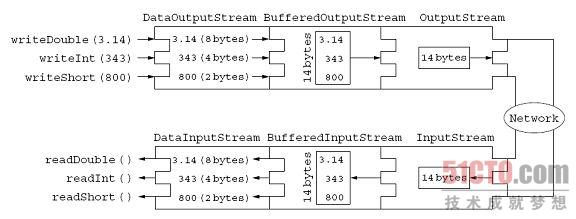
\includegraphics[scale=.8]{img/03.01.jpg}
		\caption{流组合}
		\label{fig:comp.stream}
	\end{figure}

	图3.1展示了这中组合。在这个例子中,我们先将基本数据的值,一个一个写入DataOutputStream中,DataOutputStream再将这些数据以二进制的形式写入BufferedOutputStream将三次写入的数据缓存起来,然后再由BufferedOutputStream一次性地将这些数据写入套接字的OutputStream,最后由OutputStream将数据发送到网络。在另一个终端,我们创建了相应的组合InputStream,以有效地接收基本数据类型。 

	对Java输入输出API的完整介绍不在本书的讨论范围中,不过,表3.1列出了一些相关的Java输入输出类,为介绍它们的强大功能起一个抛砖引玉的作用。Java基本输入输出类:

	Buffered[Input/Output]Stream 通过缓存性能优化

	Checked[Input/Output]Stream  维护数据检查

	Cipher[Input/Output]Stream   加密/解密 

	Data[Input/Output]Stream     数据处理 

	Digest[Input/Output]Stream   维护数据摘要 

	GZIP[Input/Output]Stream     压缩/解压缩 

	Object[Input/Output]Stream   数据处理 

	PushbackInputStream          允许一个字节或是字节是“末读的”

	PrintOutputStream            输出数据类型的字符串表示法

	Zip[Input/Output]Stream      以zip格式

\section{成帧与解析} 

	当然,将数据转换成在线路上传输的格式只完成了一半工作,在接收端还必须将接收到的字节序列还原成原始信息。应用程序协议通常处理的是由一组字段组成的离散的信息。成帧(Framing)技术则解决了接收端如何定位消息的首尾位置的问题。无论信息是编码成了文本、多字节二进制数、或是两者的结合,应用程序协议必须指定消息的接收者如何确定何时消息已完整接收。 

	如果一条完整的消息负载在一个DatagramPacket中发送,这个问题就变得很简单了:DatagramPacket 负载的数据有一个确定的长度,接收者能够准确地知道消息的结束位置。然而,如果通过TCP套接字来发送消息,情况将变得更复杂,因为TCP协议中没有消息边界的概念。如果一个消息中的所有字段都有固定的长度,同时每个消息又是由固定数量的字段组成的话,消息的长度就能够确定,接收者就可以简单地将消息长度对应的字节数读到一个byte[]缓存区中。在TCPEchoClient.java示例程序中我们就是用的这个方法,在该例中我们能从服务器获得消息的字节数。但是如果消息的长度是可变的(例如消息中包含了一些变长的文本字符串),我们事先就无法知道需要读取多少字节。 

	如果接收者试图从套接字中读取比消息本身更多的字节,将可能发生以下两种情况之一:如果信道中没有其他消息,接收者将阻塞等待,同时无法处理接收到的消息;如果发送者也在等待接收端的响应信息,则会形成死锁(deadlock);另一方面,如果信道中还有其他消息,则接收者会将后面消息的一部分甚至全部读到第一条消息中去,这将产生一些协议错误。因此,在使用TCP套接字时,成帧就是一个非常重要的考虑因素。 

	一些相同的考虑也适用于查找消息中每个字段的边界:接收者需要知道每个字段的结束位置和下一个字段的开始位置。因此,我们在此介绍的消息成帧技术几乎都可以应用到字段上。然而,最简单并使代码最简洁的方法是将这两个问题分开处理:首先定位消息的结束位置,然后将消息作为一个整体进行解析。在此我们专注于将整个消息作为一帧进行处理。

	主要有两个技术使接收者能够准确地找到消息的结束位置: 

	基于定界符(Delimiter-based):消息的结束由一个唯一的标记(unique marker,)指出,即发送者在传输完数据后显式添加的一个特殊字节序列。这个特殊标记不能在传输的数据中出现。 

	显式长度(Explicit length):在变长字段或消息前附加一个固定大小的字段,用来指示该字段或消息中包含了多少字节。 

	基于定界符的方法的一个特殊情况是,可以用在TCP连接上传输的最后一个消息上:

	在发送完这个消息后,发送者就简单地关闭(使用shutdownOutput()或close()方法)发送端的TCP连接。接收者读取完这条消息的最后一个字节后,将接收到一个流结束标记(即read()方法返回-1),该标记指示出已经读取到达了消息的末尾。 

	基于定界符的方法通常用在以文本方式编码的消息中:定义一个特殊的字符或字符串来标识消息的结束。接收者只需要简单地扫描输入信息(以字节的方式)来查找定界序列,并将定界符前面的字符串返回。这种方法的缺点是消息本身不能包含有定界字符,否则接收者将提前认为消息已经结束。在基于定界符的成帧方法中,发送者要保证满足这个先决条件。幸运的是,填充(stuffing)技术能够对消息中出现才定界符进行修改,从而是接收者不将其识别为定界符。在接收者扫描定界符时,还能识别出修改过的数据,并在输出消息中对其进行还原,从而使其与原始消息一致。这个技术的缺点是发送者和接收者双方都必须扫描消息。 

	基于长度的方法更简单一些,不过要使用这种方法必须知道消息长度的上限。发送者先要确定消息的长度,将长度信息存入一个整数,作为消息的前缀。消息的长度上限定义了用来编码消息长度所需要的字节数:如果消息的长度小于256字节,则需要1个字节;如果消息的长度小于65536字节,则需要2个字节,等等。 

	为了展示以上技术,我们将介绍下面定义的Framer接口。它有两个方法:frameMsg()方法用来添加成帧信息并将指定消息输出到指定流,nextMsg()方法则扫描指定的流,从中抽取出下一条消息。 

	\lstinputlisting[language=Java,firstline=1,lastline=12]{src/ch03/Framer.java}

	DelimFramer.java类实现了基于定界符的成帧方法,其定界符为"换行"符(\verb|"\n"|, 字节值为10)。 frameMethod()方法并没有实现填充,当成帧的字节序列中包含有定界符时,它只是简单地抛出异常。(扩展该方法以实现填充功能将作为练习留给读者)nextMsg()方法扫描流,直到读取到了定界符,并返回定界符前面的所有字符,如果流为空则返回null。如果累积了一个消息的不少字符,但直到流结束也没有找到定界符,程序将抛出一个异常来指示成帧错误。 

	\lstinputlisting[language=Java,firstline=1,lastline=50]{src/ch03/DelimFramer.java}

	1.构造函数:第14行 

	获取消息的输入流作为参数传递给该函数。 

	2.frameMsg() 方法用于添加帧信息:第18-28行 

	校验消息形式的有效性:第20-24行 

	检查消息中是否包含了定界符,如果包含,则抛出一个异常。 

	写消息:第25行 

	将成帧的消息输出到流中。 

	写定界符:第26行 

	3. nextMsg()方法从输入中提取消息:第30-48行 

	读取流中的每个字节,直到遇到定界符为止:第35行 

	处理流的终点:第36-43行 

	如果在遇到定界符之前就已经到了流的终点,则分两种情况:一是从帧的构造开始或从遇到前一个定界符以来,缓存区已经接收了一些字节,这时程序将抛出一个异常;否则nextMsg()方法将返回null以表示全部消息已接收完。 

	将无定界符的字节写入消息缓存区:第44行 

	将消息缓存区中的内容以字节数组的形式返回:第47行 

	我们的定界符帧有一个限制,即它不支持多字节定界符。如何对其进行修改以支持多字节定界符将作为练习留给我们的读者。 

	LengthFramer.java类实现了基于长度的成帧方法,适用于长度小于65535 ($2^{16}-1$)字节的消息。发送者首先给出指定消息的长度,并将长度信息以big-endian顺序存入两个字节的整数中,再将这两个字节放在完整的消息内容前,连同消息一起写入输出流。在接收端,我们使用DataInputStream以读取整型的长度信息;readFully() 方法将阻塞等待,直到给定的数组完全填满,这正是我们需要的。值得注意的是,使用这种成帧方法,发送者不需要检查要成帧的消息内容,而只需要检查消息的长度是否超出了限制。 

	\lstinputlisting[language=Java,firstline=1,lastline=57]{src/ch03/LengthFramer.java}

	1. 构造函数:

	获取帧消息源的输入流,并将其包裹在一个DataInputStream中。 

	2. frameMsg()方法用来添加成帧信息:

	校验消息长度:第22行 

	由于我们用的是长为两个字节的字段,因此消息的长度不能超过65535。(注意该值太
	大而不能存入一个short型整数中,因此我们每次只向输出流写一个字节)。 

	输出长度字段:第26-27行 

	添加长度信息(无符号short型整数)前缀,输出消息的字节数。 

	输出消息:第28行 

	3.nextMsg()方法用于从输入流中提取下一帧:第30-41行 

	读取长度前缀:第34-38行 

	readUnsignedShort()方法读取两个字节,将它们作为big-endian整数进行解释,并以int
	型整数返回它们的值。 

	读取指定数量的字节:第40-41行 

	readfully() 将阻塞等待,直到接收到足够的字节来填满指定的数组。 

	以字节的形式返回消息:第40行 


\section{Java特定编码}

	当你使用套接字时,通常要么是你需要同时创建通信信道两端的程序(这种情况下你也拥有了协议的完全控制权),要么实现一个给定的协议进行通信。如果你知道(i)通信双方都使用Java实现,而且(ii)你拥有对协议的完全控制权,那么就可以使用Java的内置工具如Serializable接口或远程方法调用(Remote Method Invocation,RMI)工具。RMI能够调用不同Java虚拟机上的方法,并隐藏了所有繁琐的参数编码解码细节。序列化(Serialization)处理了将实际的Java对象转换成字节序列的工作,因此你可以在不同虚拟机之间传递Java对象实例。

	这些能力可能就好像沟通的涅槃,但是在实际中,由于种种原因,它们并不总是最好的解决方案。首先,由于它们都是很笼统的工具,因而在通信开销上不能做到最高效。例如,一个对象的序列化形式,其包含的信息在Java虚拟机(JVM)环境以外是毫无意义的。其次,Serializable和Externalizable接口不能用于已经定义了不同传输格式的情况--如一个标准的协议。最后,用户自定义的类必须自己实现它们的序列化接口,而这项工作很容易出错。再强调一次,在某些情况下,这些Java的内置工具的确很有用,但是有些时候,"实现你自己的方法"可能更简单、容易或更有效。 


\section{构建和解析协议消息}

	本章结束时我们再看一个简单的例子,对在实现别人定义的协议时可能用到的技术进行了介绍。这个例子程序是一个简单的"投票"协议,如图3.2所示。这里,一个客户端向服务器发送了一个请求消息,消息中包含了一个候选人ID,范围是0至1000。 


	\begin{figure}[htbp]%位置选项
		\centering
		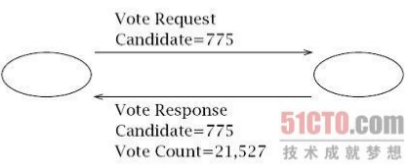
\includegraphics[scale=.8]{img/03.02.png}
		\caption{投票协议}
		\label{fig:vote.prot}
	\end{figure}

	Vote Reques:投票请求, Candidate:候选人,Vote Count:选票总数 

	程序支持两种请求。一种是查询(inquiry),即向服务器询问给定候选人当前获得的投票总数。服务器发回一个响应消息,包含了原来的候选人ID和该候选人当前(查询请求收到时)获得的选票总数。另一种是投票(voting)请求,即向指定候选人投一票。服务器对这种请求也发回响应消息,包含了候选人ID和其获得的选票数(包括了刚投的一票)。 

	在实现一个协议时,定义一个专门的类来存放消息中所包含的信息是大有裨益的。该类提供了操作消息中的字段的方法--同时用来维护不同字段之间的不变量。在我们的例子中,客户端和服务器端发送的消息都非常简单,它们唯一的区别是服务器端发送的消息包含了选票总数和一个表示响应消息(不是请求消息)的标志。因此,我们可以用一个类来表示客户端和服务器端的两种消息。VoteMsg.java类展示了每条消息中的基本信息: 

	布尔值isInquiry,其值为true时表示该消息是查询请求(为false时表示该消息是投票信息); 

	布尔值isResponse,指示该消息是响应(由服务器发送)还是请求;

	整型变量candidateID指示了候选人的ID; 

	长整型变量voteCount指示出所查询的候选人获得的总选票数。 

	这个类还维护了以下字段间的不变量: 

	candidateID的范围是0到1000。 

	voteCount在响应消息中只能是一个非零值(isResponse为true)。 

	voteCount 不能为负数。 

	\lstinputlisting[language=Java,firstline=1]{src/ch03/VoteMsg.java}

	现在我们有了一个用Java表示的投票消息,还需要根据一定的协议来对其进行编码和解码。VoteMsgCoder接口提供了对投票消息进行序列化和反序列化的方法。 

	\lstinputlisting[language=Java,firstline=1]{src/ch03/VoteMsgCoder.java}

	toWire()方法用于根据一个特定的协议,将投票消息转换成一个字节序列,fromWire()方法则根据相同的协议,对给定的字节序列进行解析,并根据信息的内容构造出消息类的一个实例。 

	为了介绍不同的信息编码方法,我们展示了两个实现VoteMsgCoder接口的类。一个使用的是基于文本的编码方式,另一个使用的是二进制的编码方式。如果你能确定一直不变地使用一种编码方式,那么toWire()方法和fromWire()方法就可以定义为VoteMsg类的一部分。这里我们这样做是为了强调抽象表示与编码的细节是相互独立的。 


	\subsection{基于文本的表示方法}

		首先,我们介绍一个用文本方式对消息进行编码的版本。该协议指定使用US-ASCII字符集对文本进行编码。消息的开头是一个所谓的"魔术字符串",即一个字符序列,用于接收者快速将投票协议的消息和网络中随机到来的垃圾消息区分开。投票/查询布尔值被编码成字符形式,'v'表示投票消息,'i'表示查询消息。消息的状态,即是否为服务器的响应,由字符'R'指示。状态标记后面是候选人ID,其后跟的是选票总数,它们都编码成十进制字符串。VoteMsgTextCoder类提供了一种基于文本的VoteMsg编码方法。 

		\lstinputlisting[language=Java,firstline=1]{src/ch03/VoteMsgTextCoder.java}

		toWire()方法简单地创建一个字符串,该字符串中包含了消息的所有字段,并由空白符隔开。fromWire()方法首先检查"魔术"字符串,如果在消息最前面没有魔术字符串,则抛出一个异常。这里说明了在实现协议时非常重要的一点:永远不要对从网络来的任何输入进行任何假设。你的程序必须时刻为任何可能的输入做好准备,并能够很好地对其进行处理。在这个例子中,如果接收到的不是期望的消息,fromWire()方法将抛出一个异常,否则,就使用Scanner实例,根据空白符一个一个地获取字段。注意,消息的字段数与其是请求消息(由客户端发送)还是响应消息(由服务器发送)有关。如果输入流提前结束或格式错误,fromWire()方法将抛出一个异常。 

	\subsection{二进制表示方法} 

		下面我们将展示另一种对投票协议消息进行编码的方法。与基于文本的格式相反,二进制格式使用固定大小的消息。每条消息由一个特殊字节开始,该字节的最高六位为一个"魔术"值010101。这一点少量的冗余信息为接收者收到适当的投票消息提供了一定程度的保证。该字节的最低两位对两个布尔值进行了编码。消息的第二个字节总是0,第三、第四个字节包含了candidateID值。只有响应消息的最后8个字节才包含了选票总数信息。 

		\lstinputlisting[language=Java,firstline=1]{src/ch03/VoteMsgBinCoder.java}

		就像在第3.1.1节中一样,我们创建了一个ByteArrayOutputStream并将其包裹在一个DataOutputStream中来接收结果。这个编码方法利用了在合法candidateID中,其最高两个字节始终为0的特点。还要注意的是,该方法通过使用按位或操作,使用1位对每个布尔值进行编码。 

	\subsection{发送和接收} 

		通过流发送消息非常简单,只需要创建消息,调用toWire()方法,添加适当的成帧信息,再写入流。当然,接收消息就要按照相反的顺序执行。这个过程适用于TCP协议,而对于UDP协议,不需要显式地成帧,因为UDP协议中保留了消息的边界信息。为了对发送与接收过程进行展示,我们考虑投票服务的如下几点:1)维护一个候选人ID与其获得选票数的映射,2)记录提交的投票,3)根据其获得的选票数,对查询指定的候选人和为其投票的消息做出响应。首先,我们实现一个投票服务器所用到的服务。当接收到投票消息时,投票服务器将调用VoteService类的handleRequest() 方法对请求进行处理。 


		\lstinputlisting[language=Java,firstline=1]{src/ch03/VoteService.java}

		1.创建候选人ID与选票数量的映射:第9行 

		对于查询请求,给定的候选人ID用来在映射中查询其获得的选票数量。对于投票请求,增加后的选票数又存回映射。 

		2.handleRequest():第11-27行 

		返回响应:第12-14行 

		如果投票消息已经是一个响应信息,则直接发回而不对其进行处理和修改。否则,对其响应消息标志进行设置。 

		查找当前获得的选票总数:第16-21行 

		根据候选人ID从映射中获取其获得的选票总数。如果该候选人ID在映射中不存在,则将其获得的选票数设为0。 

		如果有新的投票,则更新选票总数:第12-24行 

		如果之前候选人不存在,则创建新的映射,否则,只是简单地修改已有的映射。 

		设置选票总数并返回消息:第25-26行 

		下面我们将展示如何实现一个TCP投票客户端,该客户端通过TCP套接字连接到投票服务器,在一次投票后发送一个查询请求,并接收查询和投票结果。 

		\lstinputlisting[language=Java,firstline=1]{src/ch03/VoteClientTCP.java}

		1.参数处理:第12-18行 

		2.创建套接字,获取输出流:第20-21行 

		3.创建二进制编码器和基于长度的成帧器:第23-26行 

		我们将使用一个编码器对投票消息进行编码和解码,这里为我们的协议选择的是二进制编码器。其次,由于TCP协议是一个基于流的服务,我们需要提供字节的帧。在此,我们使用LengthFramer类,它为每条消息添加一个长度前缀。注意,我们只需要改变具体的类,就能方便地转换成基于定界符的成帧方法和基于文本的编码方式,这里将VoteMsgCoder和Framer换成VoteMsgTextCoder和DelimFramer即可。 

		4.创建和发送消息:第28-43行 

		创建,编码,成帧和发送查询请求,后面是为相同候选人的投票消息。 

		5.获取和解析响应:第45-56行 

		我们使用nextMsg()方法用于返回下一条编码后的消息,并通过fromWire()方法对其进行解析/解码。 

		6.关闭套接字:第58行 

		下面我们示范TCP版本的投票服务器。该服务器反复地接收新的客户端连接,并使用VoteService类为客户端的投票消息作出响应。 

		\lstinputlisting[language=Java,firstline=1]{src/ch03/VoteServerTCP.java}

		1.为服务器端建立编码器和投票服务:第20-21行 

		2.反复地接收和处理客户端连接:第23-46行 

		接收新的客户端,打印客户端地址:第24-25行 

		为客户端创建成帧器:第28行 

		从客户端获取消息并对其解码:第30-38行 

		反复地向成帧器发送获取下一条消息的请求,直到其返回null,即指示了消息的结束。 

		处理消息,发送响应信息:第34-37行 

		将解码后的消息传递给投票服务,以进行下一步处理。编码,成帧和回发响应消息。 

		UDP版本的投票客户端与TCP版本非常相似。需要注意的是,在UDP客户端中我们不需要使用成帧器,因为UDP协议为我们维护了消息的边界信息。对于UDP协议,我们使用基于文本的编码方式对消息进行编码,不过只要客户端与服务器能达成一致,也能够很方便地改成其他编码方式。 

		\lstinputlisting[language=Java,firstline=1]{src/ch03/VoteClientUDP.java}

		1.设置DatagramSocket 和连接:

		通过调用connect()方法,我们不必1)为发送的每个数据报文指定远程地址和端口,也不必2)测试接收到的每个数据报文的源地址。 

		2.创建选票和编码器:

		这次使用的是文本编码器,但我们也可以很容易地换成二进制编码器。注意这里我们不需要成帧器,因为只要每次发送都只有一个投票消息,UDP协议就已经为我们保留了边界信息。 

		3.向服务器发送请求消息:

		4.接收,解码和打印服务器响应信息:第36-45行 

		在创建DatagramPacket时,我们需要知道消息的最大长度,以避免数据被截断。当然,在对数据报文进行解码时,我们只使用数据报文中包含的实际字节,因此调用了Arrays.copyOfRange()方法来复制返回的数据报文中数组的子序列。 

		最后是UDP投票服务器,同样,也与TCP版本非常相似。 

		\lstinputlisting[language=Java,firstline=1]{src/ch03/VoteServerUDP.java}

		1.设置:

		为服务器创建接收缓存区,编码器,以及投票服务。 

		2.反复地接收和处理客户端的投票消息:

		为接收数据报文创建DatagramPacket:

		在每次迭代中将数据区重置为输入缓存区。 

		接收数据报文,抽取数据:

		UDP替我们完成了成帧的工作! 

		解码和处理请求:

		服务将响应返回给消息。 

		编码并发送响应消息:

\section{结束} 

	我们已经看到如何将基本数据类型表示成字节序列"在信道"上传输。我们还考虑了一些微妙的文本字符串编码方法,以及一些成帧和消息解析的基本方法。我们还见到了基于文本编码和二进制编码的协议的例子。 

	这里可能值得重申一下我们在前言中所说的:本章并不会使你成为专家!那需要大量的经验。但是本章中的代码能够作为你进一步探索的起点。 

